\chapter{Experiments and results}
In this chapter we will analyze the efficiency of the functions involved in the \verb|ClustAssess| package. The benchmarks were performed on a Linux server of the Core Bioinformatics group at the Cambridge Stem Cell institute. We note that the stability pipeline and ECS calculation can be performed on devices for personal use.

\section{ECS optimization results}
We stated in the previous chapter that the ECS calculation is optimized in the \verb|ClustAssess| package by computing only the $n \times m$ unique values, where $n$ and $m$ are the number of clusters of the two partitions. In this section we will compare the performance of the \verb|ClustAssess| and the \verb|clusim| packages.

\subsection{Benchmark datasets}
For benchmarking we used artificial datasets which consists of two-dimensional points which were randomly generated using the uniform distribution. The number of points varies from 50 up to 90 000, in order to capture the scalability of the two packages and test the ability to handle big data from industry. The points are clustered using the kmeans algorithm. We used the implementation from the R \verb|stats| \footnote{Documentation can be found here: \url{https://stat.ethz.ch/R-manual/R-devel/library/stats/html/kmeans.html}} package. For the first side of the experiments, we set the number of clusters to 20, but for the second experiment we varied $k$ from 5 to 1000.

\subsection{Time comparison}
First, we compare how fast is the ECS score calculated on both packages. We perform each test 30 times and use the median for comparison. To measure the time execution for \verb|clusim|, we used the \verb|timeit| Python module \footnote{Official documentation page: \url{https://docs.python.org/3/library/timeit.html}}. For \verb|ClustAssess|, we used the \verb|microbenchmark| package \footnote{Official GitHub repository: \url{https://github.com/joshuaulrich/microbenchmark}}.

Figure \ref{fig:comp-time} illustrates the time (measured in seconds) required to execute the same task on both packages. The exact values of the experiments can be found in Table \ref{tab:comp-time}. We notice how \verb|clusim| is faster than \verb|ClustAssess| for the smallest dataset but, as more points are added, the latter is getting more efficient. We notice that \verb|ClustAssess| has a linear grow proportionate to the number of points, whereas the time of execution of \verb|clusim| is increased exponentially. This behaviour confirms the expectation raised from the previous chapter, where we stated that calculating only the unique values should bring performance boosts.


\begin{figure}[H]
    \centering
    \makebox[\textwidth][c]{
        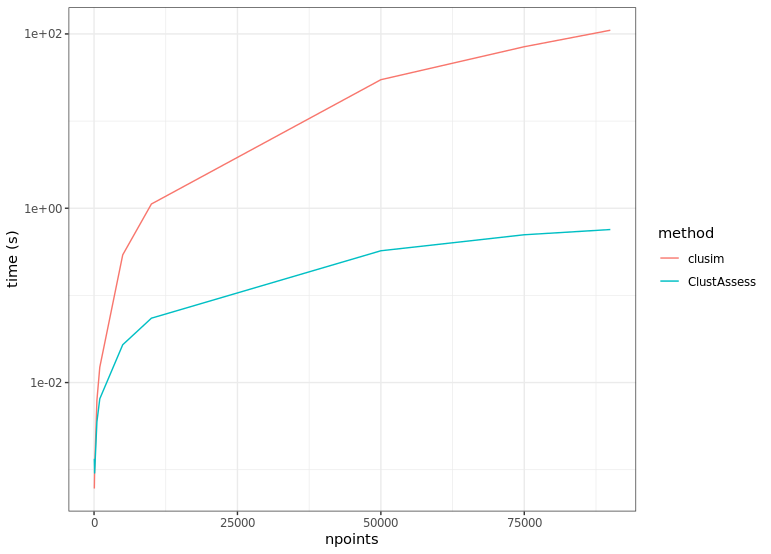
\includegraphics[width=0.7\linewidth]{images/ch4/4_clusim_ca_time.png}
    }
    \caption{\label{fig:comp-time}\textbf{Runtime comparison between ClustAssess and clusim.} The results are displayed on logarithmic scale.}
\end{figure}


\begin{table}[]

\resizebox{\textwidth}{!}{
\begin{tabular}{|l||l|l|l|l|l|l|l|l|l|}
\hline
                     & \textbf{50} & \textbf{100} & \textbf{500} & \textbf{1000} & \textbf{5 000} & \textbf{10 000} & \textbf{50 000} & \textbf{75 000} & \textbf{90 000} \\ \hline \hline
\textbf{ClustAssess} & 0.001335    & 0.000918     & 0.003551     & 0.006514      & 0.027171       & 0.054795        & 0.325342        & 0.496565        & 0.57            \\ \hline
\textbf{clusim}      & 0.000608    & 0.000995     & 0.006256     & 0.015005      & 0.291919       & 1.119508        & 29.86761        & 71.3589         & 110.3293        \\ \hline
\end{tabular}}
\caption{\label{tab:comp-time} Runtime of ClustAssess and clusim on datasets with various sizes, measured in seconds.}
\end{table}

\subsection{Memory consumption comparison}
For analyzing the memory consmuption, we will proceed in a similar manner. We will use the \verb|memory_profiler| module \footnote{Official GitHub repository: \url{https://github.com/pythonprofilers/memory_profiler}} for \verb|clusim|, and the \verb|profvis| package \footnote{Official GitHub repository: \url{https://github.com/rstudio/profvis}} for \verb|ClustAssess|. At each run, we will extract the maximum memory allocation that has occured during the execution.

Figure \ref{fig:comp-mem} illustrates the allocated memory (measure in GiB) during the execution of the task. It is noticeable that \verb|ClustAssess| is memory efficient and requires only a few MiB of memory. On the other side, \verb|clusim| shows the disadvantages of storing the whole affinity matrix into memory: already for 10 000 points the 1 GiB threshold is surpassed (see \ref{tab:comp-mem}) and as the dataset increases, the memory usage also increases exponentially, up to a value of 241 GiB of memory to calculate the ECS of two partitions with 90 000 points.
We note that, at the time of writing, the machines used in daily tasks have between 8 and 32 GB of memory \footnote{Various sources such as \href{https://www.crucial.com/articles/about-memory/how-much-ram-does-my-computer-need}{Crucial} - a memory stick fabricator - indicate that the average user needs between 8 and 16 GB of RAM.}. Therefore, the \verb|clusim| package doesn't scale on big datasets and cannot be used by the casual user.

\begin{figure}[H]
    \centering
    \makebox[\textwidth][c]{
        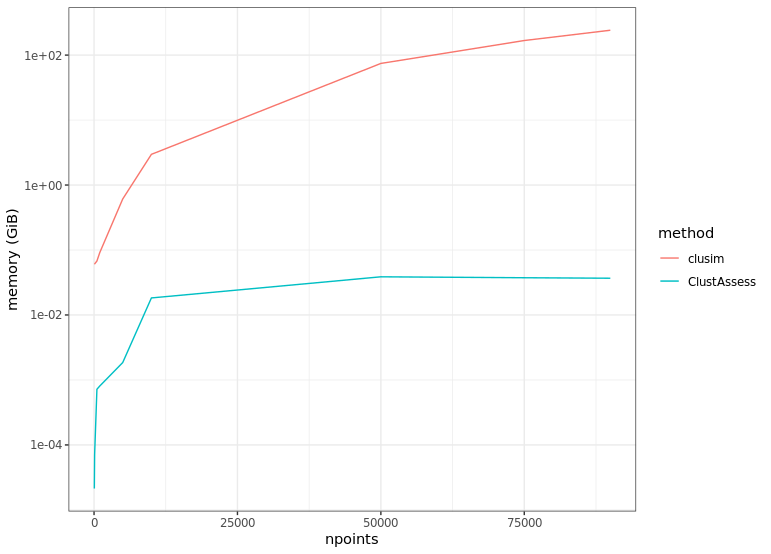
\includegraphics[width=0.7\linewidth]{images/ch4/4_clusim_ca_memory.png}
    }
    \caption{\label{fig:comp-mem}\textbf{Memory consumption comparison between ClustAssess and clusim.} The results are displayed on logarithmic scale.}
\end{figure}


\begin{table}[]

\resizebox{\textwidth}{!}{
\begin{tabular}{|l||l|l|l|l|l|l|l|l|l|}
\hline
                     & \textbf{50} & \textbf{100} & \textbf{500} & \textbf{1000} & \textbf{5 000} & \textbf{10 000} & \textbf{50 000} & \textbf{75 000} & \textbf{90 000} \\ \hline \hline
\textbf{ClustAssess} & 0.000021 & 0.000071 & 0.000719 & 0.000808 & 0.001855 & 0.018308 & 0.038693 & 0.037435 & 0.036799 \\ \hline
\textbf{clusim}      & 0.060688 & 0.061069 & 0.06767 & 0.091365 & 0.610633 & 2.970745 & 74.46173 & 167.6854 & 241.5057 \\ \hline
\end{tabular}}
\caption{\label{tab:comp-mem} Memory consumption of ClustAssess and clusim on datasets with various sizes, measured in GiB.}
\end{table}

\subsection{The impact of the number of clusters}
\verb|ClustAssess| seem to have an efficient way of calculating the Element-Centric Similarity score by using small amounts of memory, but the question is whether its approach scales well on a larger number of clusters. To benchmark its behaviour, we will use the dataset with 90 000 points and vary the number of clusters as described in the previous section.

Figure \ref{fig:comp-k} shows a behaviour that was expected for \verb|ClustAssess|: increasing the number of clusters leads to more unique values to be calculated, hence more execution time required (see the left panel). As for the memory consumption (the right panel), we notice a slight increase that still remains under the threshold of 100 MiB.

Contrary to the expectations, \verb|clusim| seems to perform better when the number of clusters is increased (from 122 seconds for $k = 5$ to 77 for $k = 1000$). Even with this improvement, it still performs worse than \verb|ClustAssess|, which takes 50 seconds to calculate the ECS for $k = 1000$.

\begin{figure}[H]
    \centering
    \makebox[\textwidth][c]{
        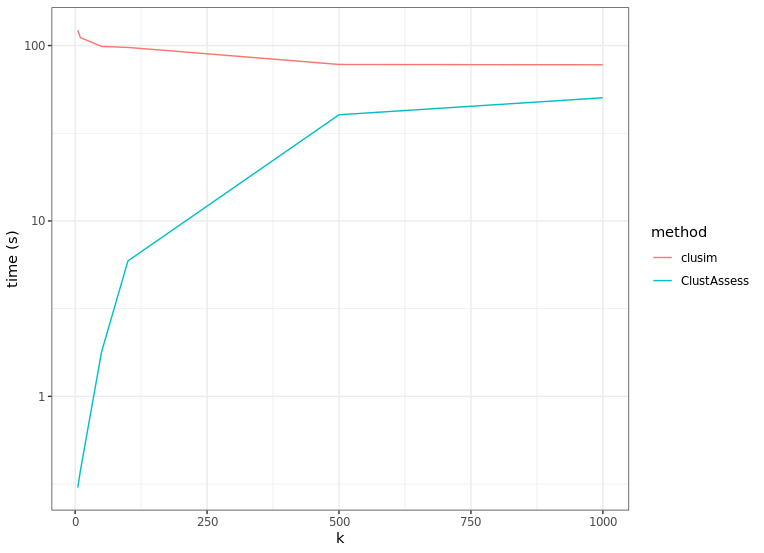
\includegraphics[width=0.5\linewidth]{images/ch4/4_clusim_ca_time_k.png}
        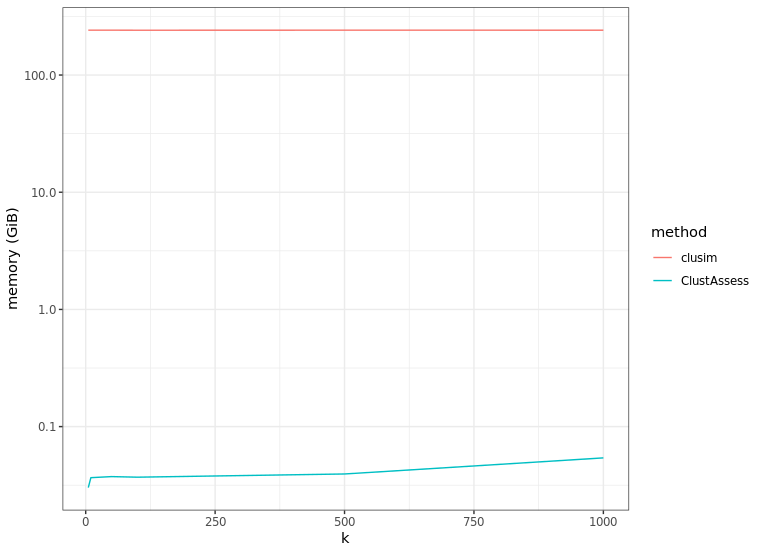
\includegraphics[width=0.5\linewidth]{images/ch4/4_clusim_ca_memory_k.png}
    }
    \caption{\label{fig:comp-k}\textbf{Runtime (left) and memory consumption (right) comparison between ClustAssess and clusim when different number of clusters are used}.}
\end{figure}

\subsection{Results accuracy}
The final task is to compare the ECS scores obtained by both packages. Calculating the median of the absolute difference results in an average difference of $5.20417e-17$, which is a negligible difference closer to the machine precision. This leads to the conclusion that the optimization did not affect the accuracy of the ECS results.

\subsection{On the scalability of ClustAssess}
Given the results presented above and the accuracy of the results, the optimized version presented in \verb|ClustAssess| for calculating the ECS score should be considered a more suitable choice, as it is more efficient (especially for a reasonable number of clusters) and it scales linearly as the dataset increases. Also, the low memory consumption is another strong point that highlights the advantages of using our package.

\section{Stability pipeline performance}
Given that for the stability pipeline multiple requires multiple runs of the clustering, an assessment of its scalability and efficiency is required. This section will contain only the analysis of the time execution. Given the memory consumption results from the previous section, we chose not to include additional memory benchmark, as ECS proved to scale well regarding the required space.

Informations regarding the time of executing the whole stability pipeline can also be found at the end of the \href{https://core-bioinformatics.github.io/ClustAssess/articles/stability-based-parameter-assessment.html}{vignette} of the \verb|ClustAssess| package.

\subsection{Benchmark dataset}
The pipeline will be applied on the Mende dataset \cite{Mende2022} which contains a total number of 13 099 cells. The dataset will be subsampled to the following sizes: 1319, 3297, 4396, 6594 and 13099. 

The number of different seeds (or of the runs) will be 30.

\subsection{Benchmark guidelines}
The plots presented in the third chapter are based on object that are created inside the stability pipeline and which contain fields related to the list of partitions, their frequency, the ECC. There are five independent functions that create objects inside the stability pipeline:
\begin{itemize}
    \item \verb|feature_stability|: the object is used for all plots for the Dimensionality reduction step;
    \item \verb|nn_n_conn_comps|: the object is used to create the Connected components target plot from the Graph construction step;
    \item \verb|nn_importance|: the object is used to create the other plots from the same step;
    \item \verb|clustering_importance|: the object is used to create the first two plots related to choosing the community detection algorithm from the Clustering step;
    \item \verb|resolution_importance|: the object is used to create the last two type of plots from the same step.
\end{itemize}

All functions (with the exception of \verb|nn_n_conn_comps|) require the merging of partitions in order to speed up the calculation of the ECC score and to enable the identification of the most frequent partition. Thus, an additional parameter will be the ECS threshold (see Section \ref{sec:part-merge}).

Also, in Section \ref{sec:paral} we mentioned that \verb|ClustAssess| offers support for parallelization. Therefore, the following benchmark will try to evaluate the performance of the five functions with different values for the ECS threshold and the number of cores.

\subsection{Benchmark results}
The results, visually presented in Figure \ref{fig:pipeline-benchmark}, lead to multiple conclusions. First, \\ \verb|nn_n_conn_comps| not only is running fast, but also scales very good as the dataset size increases. The plots are in logarithmic scale, thus looking at panel B, the last row, we can draw the conclusion that the behaviour of this function is sublinear. We can also remark that increasing the number of parallel processes brings significant improvements to the runtime.

The \verb|feature_stability|, \verb|nn_importance| and \verb|clustering_importance| present a similar behaviour, as the panel A of the same figure suggests. One reason might be that the first two contain repeated calls to the dimensional reduction methods, which are computationally expensive. Also, compared to the \verb|nn_n_conn_comps| method, a graph clustering algorithm is applied instead of a method that identifies the connected components. The similar behaviour for the function \verb|clustering_importance| might be explained by the fact that it performs multiple clustering algorithm in a single iteration. Also, SLM usually requires significantly more time to run than the other methods.

The \verb|resolution_importance| function performs better, as it doesn't require any call to a dimensional reduction method and it uses a single clustering algorithm. One thing that is common to the four methods is how they behave when increasing the number of cores. Until a certain point, using multiple processes has a significant gain to the overall execution of the pipeline. However, there is the risk of creating an overhead by adding too many cores. The behaviour is easily noticed in the second Panel for the smallest dataset (red colour): the performance is worsened because the back and forth transfer between the main process and the newly created R instances require more time than the execution of the instances themselves. This happens more frequently when the data is small enough for a run to be executed pretty fast. In the panel B we can observe that if the number of points is increased, the number of situation of performance drops caused by overheads decreases.

As for the ECS threhsold, lowering the threshold to obtain less partitions doesn't seem to help in improving the performance. The reason behind this is that the process of identification of similar partitions that could be merged currently requires the running of pairwise ECS calculation, so the comparison saved after merged are used to obtain the merging.


\begin{figure}[H]
    \centering
    \makebox[\textwidth][c]{
        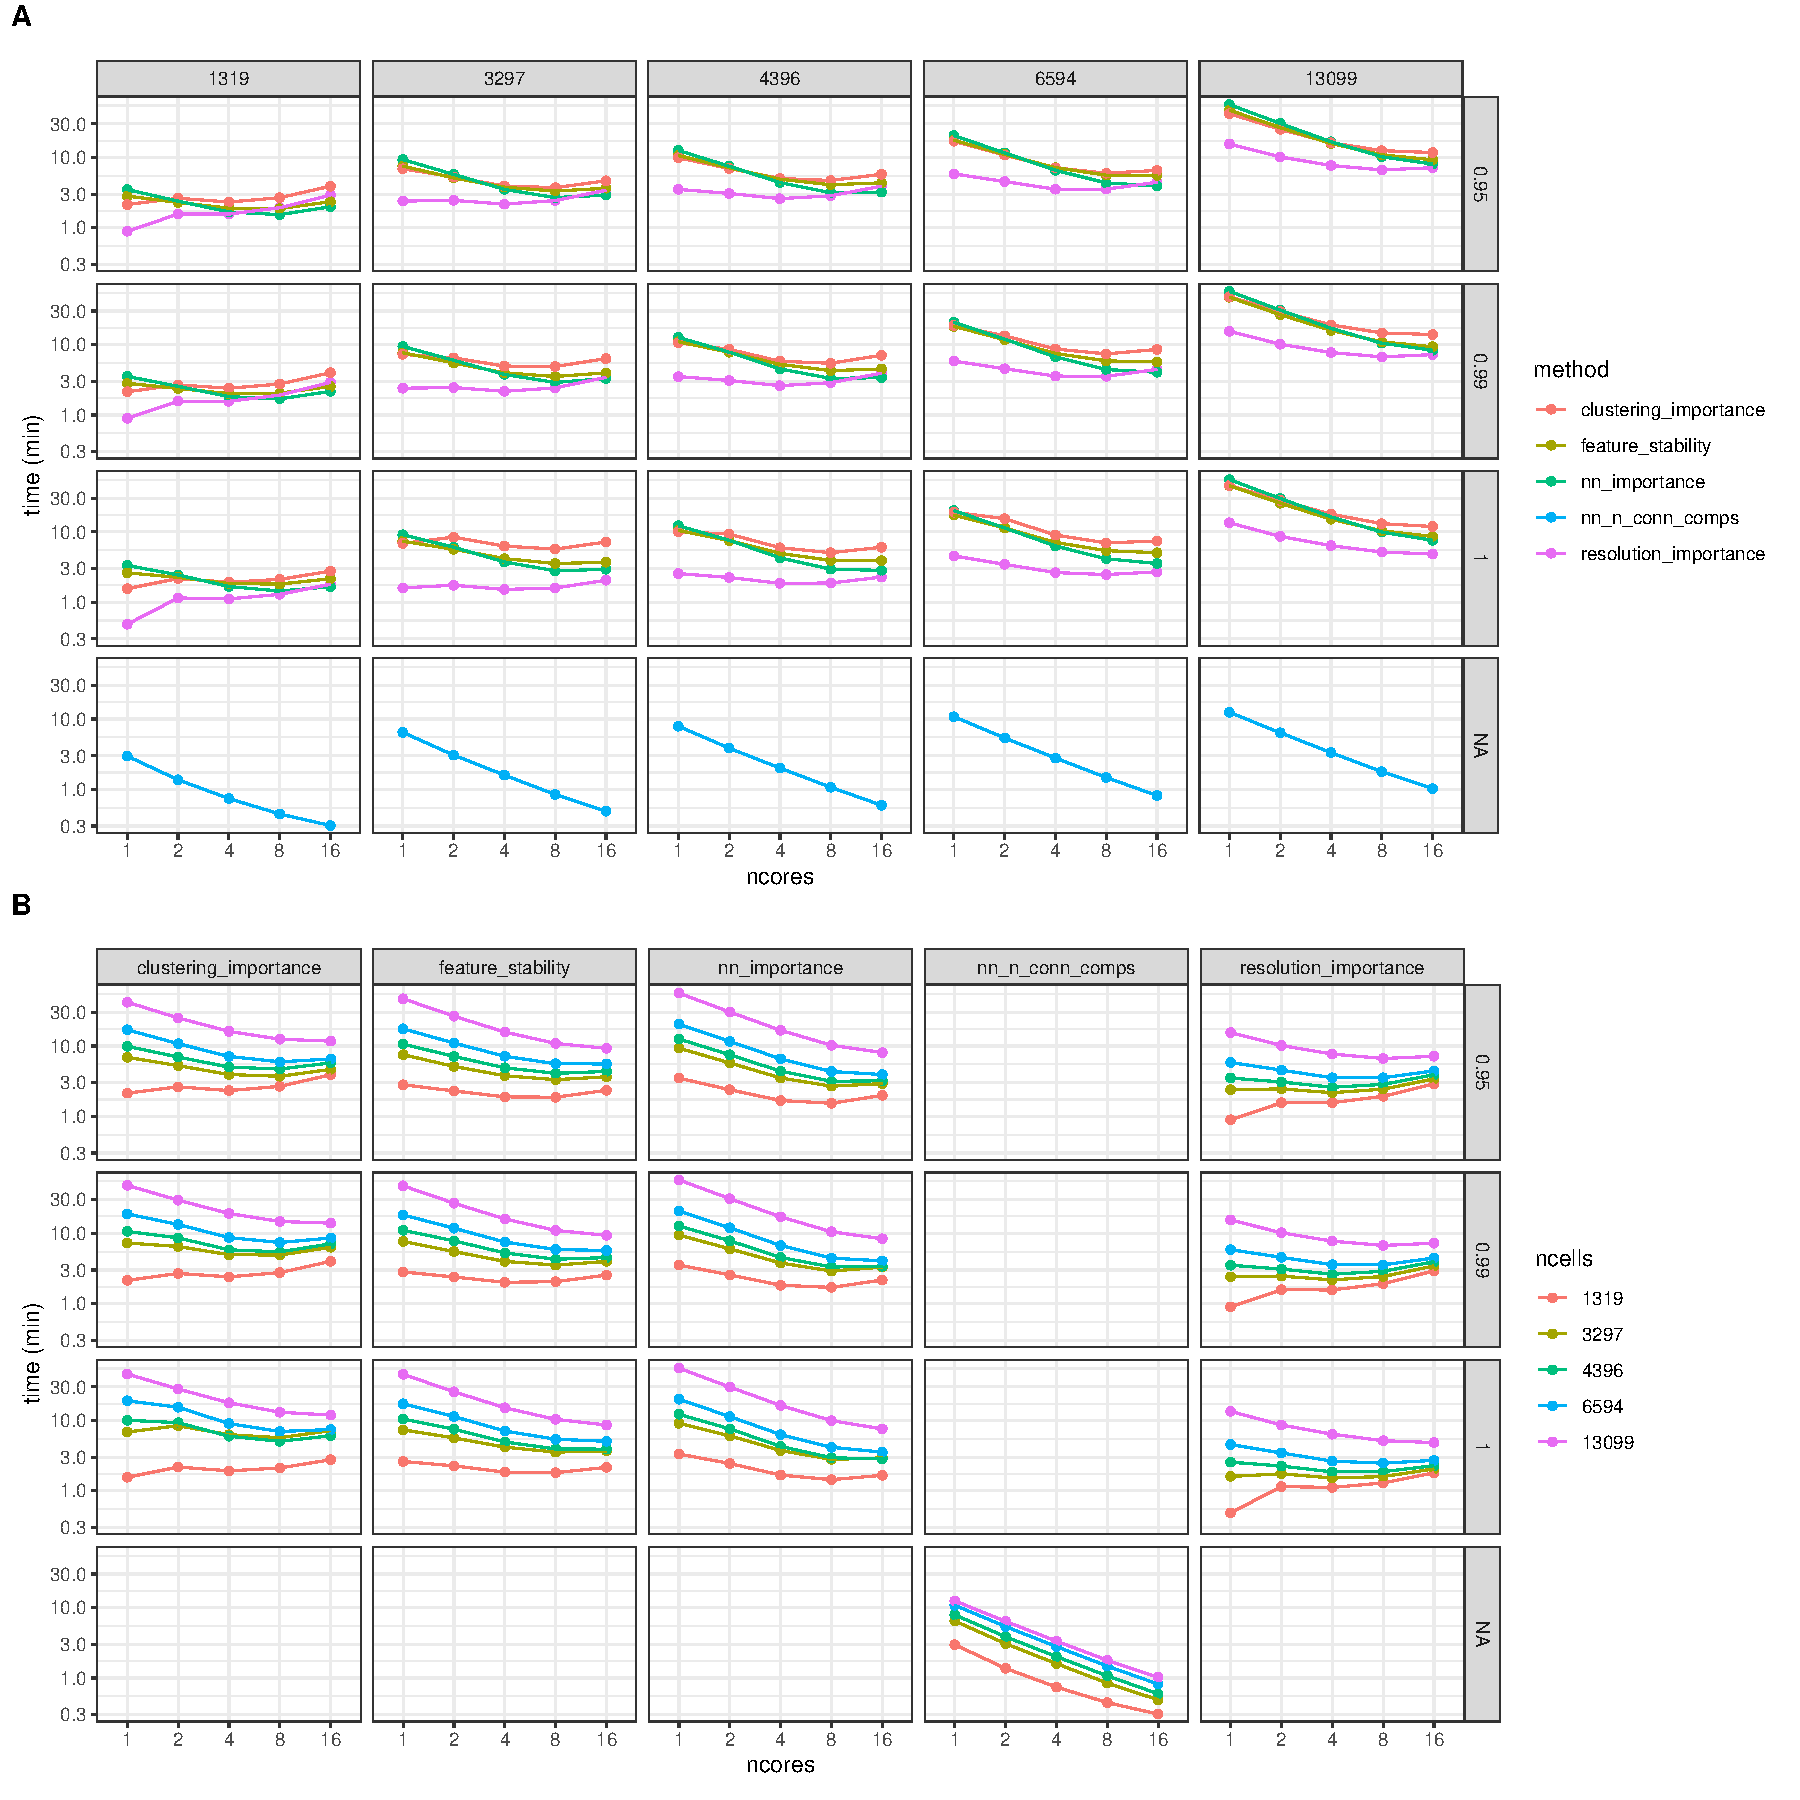
\includegraphics[width=\linewidth]{images/ch4/4_pipeline_benchmark.pdf}
    }
    \caption{\label{fig:pipeline-benchmark}\textbf{Time benchmarks for individual steps of the ClustAssess data-driven evaluation of parameters with respect to the number of cells, ECS thresholds, and number of cores.}
A. Assessment of runtime for an incremental number of cells (columns, corresponding to 10\%, 25\%, 33\%, 50\%, 100\% of the full dataset), subsampled using geometric sketching. The agreement-threshold is controlled via the ECS threshold (rows, the NA row corresponds to the \texttt{nn\_n\_conn\_comps}, as no clustering is performed). On the x-axis we represent the number of cores; the y-axis summarises the runtime (seconds). The colours indicate the methods used to evaluate some parameters of the graph-based clustering pipeline: \texttt{feature\_stability} (the importance of the feature set used as input for the dimensionality reduction), \texttt{nn\_importance} and \texttt{nn\_n\_conn\_comps} (the importance of the base embedding, the number of neighbours and the graph type, graph construction step), \texttt{clustering\_importance} and \texttt{resolution\_importance} (the effect of the clustering method and resolution parameter, community detection step). 
B. Assessment of runtime presented from the perspective of individual methods. We note that the 
%resolution step is minimally affected by the number of cells, whereas the 
runtime increases with more cells; moreover the parallelisation substantially speeds up the processing. Changes in the ECS threshold do not have an impact on runtime.}

\end{figure}

\subsection{Interpreting the results}
The conclusion is that the stability pipeline has scaling capabilities and can be run in a reasonable amount of time for medium-sized datasets. The performance differ from dataset to dataset and could be affected by factors such as:
\begin{itemize}
    \item the clustering algorithm that is used: Louvain and Louvain refined are generally faster than Leiden and SLM (at least in the Seurat's implementation);
    \item the size of the dataset: to obtain the stability plots in a reasonable amount of time, we advise performing a subsampling before running the pipeline;
    \item the number of cores: although it is expected that increasing the number of cores would benefit the performance, there are situations when it could worsen the runtime because of the overheads. A recommendation would be using a number of cores that would lead to a reasonable split of all the runs (if there is a total of 32 runs and we set the number of cores to 16, there is a high chance of reaching the overhead). Also, for smaller datasets each run is executed faster, therefore the overhead threshold will vary depending on the size of the provided data.
\end{itemize}